% $Log$
% Revision 1.3  2006/01/06 17:51:53  kelsaka
% - Rechtschreibkorrekturen
%
% Revision 1.2  2006/01/03 16:45:21  kelsaka
% - korrekturen eingepflegt: v. a. n�here definition der iterationsschritte
%
% Revision 1.1  2006/01/03 10:37:55  kelsaka
% - move to folder proposal
%
% Revision 1.1  2005/12/30 15:16:19  kelsaka
% initial creation
% 

\begin{titlepage}


\begin{tabular} {p{0.50\textwidth} p{0.50\textwidth}}
\begin{flushleft}
	
\includegraphics[width=0.45\textwidth]{image/logo-uni-ol.pdf}
\end{flushleft}
 &
\begin{center}
	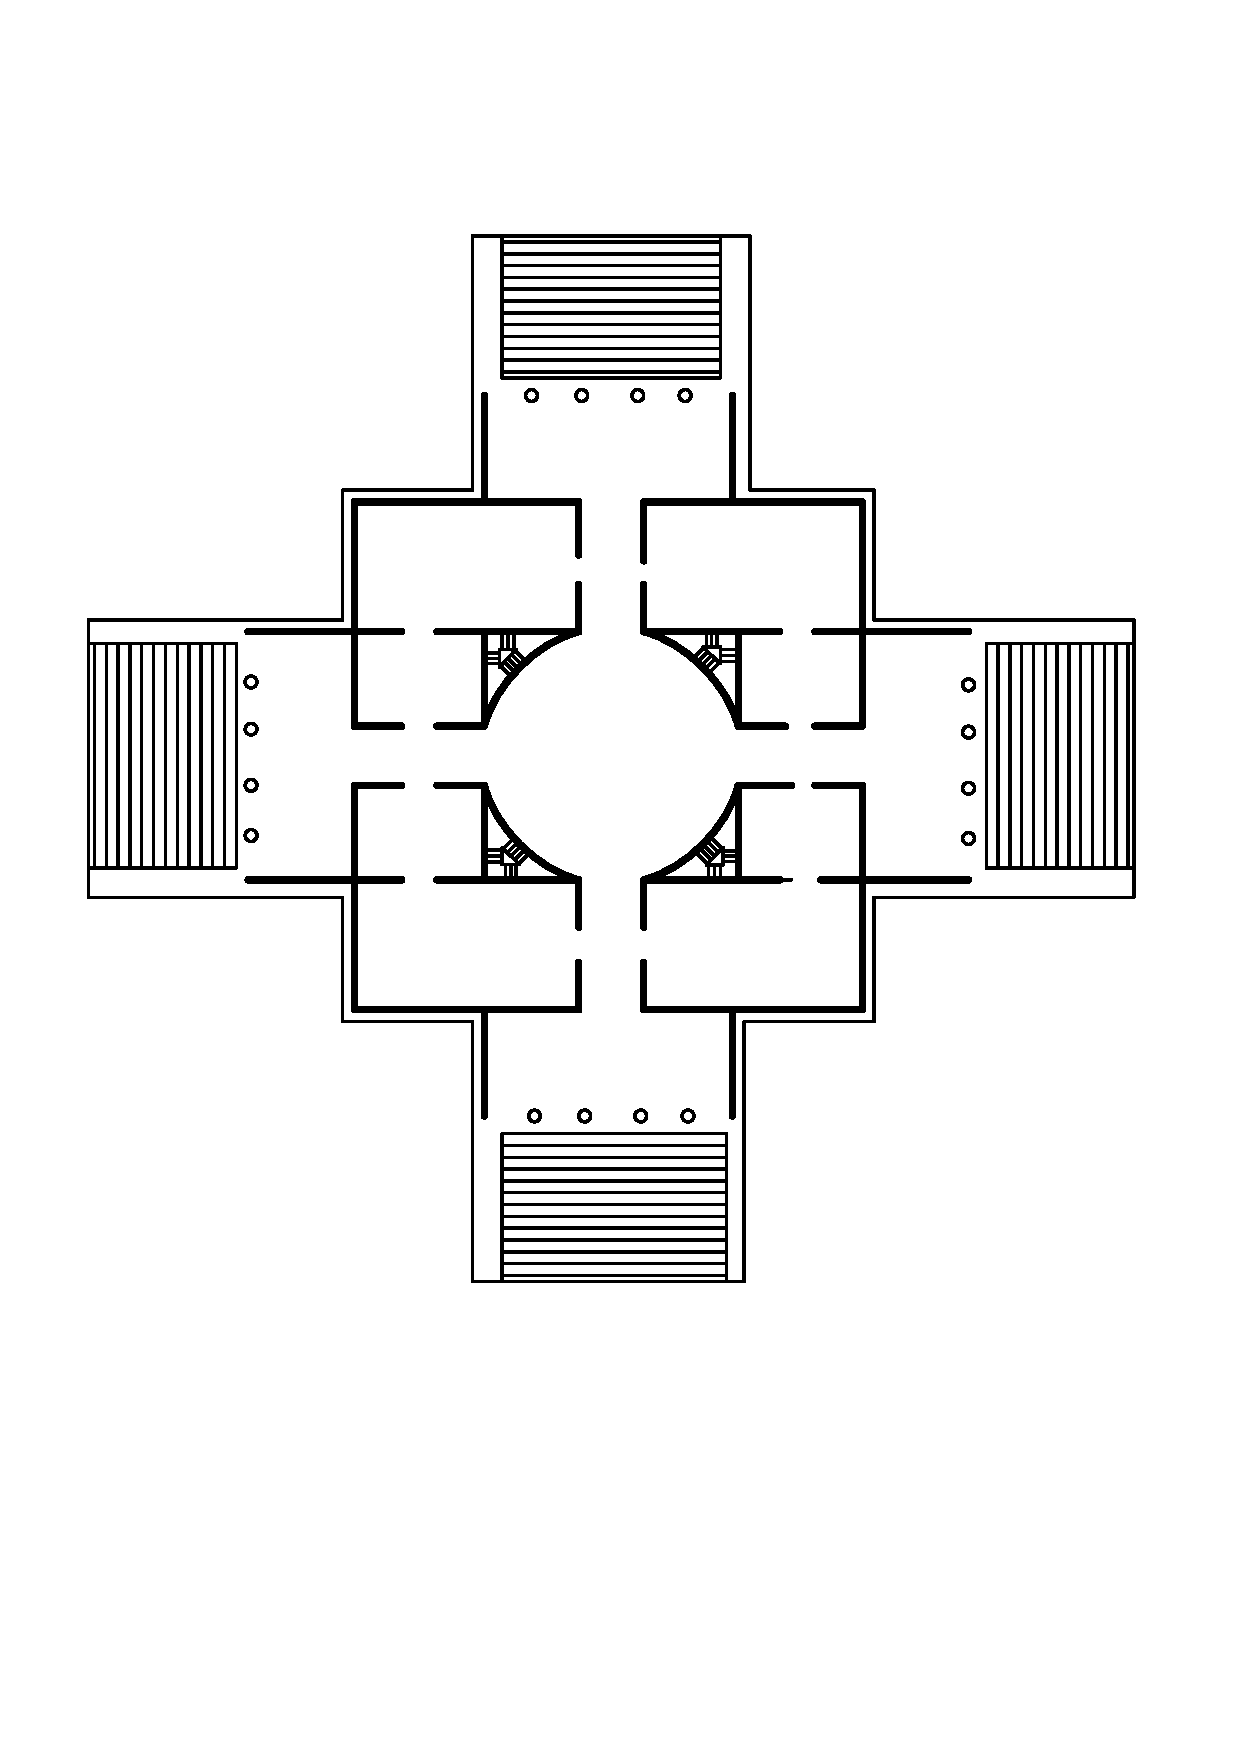
\includegraphics[width=0.15\textwidth]{image/Palladio-Logo-03.pdf}
\end{center}
\end{tabular}

\begin{center}

\vfill {\ \\ \ \\ \ \\}

\vfill {\large{Proposal einer Diplomarbeit}}

\vfill {\large \normalfont --------------------------------------------------------------------------------------------\\
\textsc{\LARGE Entwicklung und Transformation \\ \tiny $\,$ \\ \LARGE eines EMF-Modells des \\ \tiny $\,$ \\ \LARGE Palladio Komponenten-Meta-Modells \ \\
\large \normalfont --------------------------------------------------------------------------------------------}}

\vfill {\ \\ \ \\ \ \\ \ \\ \ \\ \ \\ \ \\ \ \\ \ \\ \ \\}


\vfill{
\begin{flushleft}
\textbf{Bearbeitet von:} \\
Klaus Krogmann \\
Reinekeweg 2 \\
26676 Harkebr�gge \\
\texttt{kelsaka@gmx.de}
\end{flushleft}
}

\vfill {
\begin{flushleft}
\textbf{Betreut von:} \\
Erstgutachter: Jun.-Prof. Dr. Ralf Reussner \\
Zweitgutachter: Prof. Dr. Wilhelm Hasselbring \\
Betreuer: Dipl.-Wirtsch.-Inform. Steffen Becker \\
Fk. II, Department f�r Informatik, Abt. Software Engineering\\
an der Carl-Von-Ossietzky Universit�t, Oldenburg
\end{flushleft}
}

\vfill 
\begin{flushleft}
	\begin{tabular}{l}
				$$Revision$$\\
				$$Date$$ \\
				Status: Release
	\end{tabular}
\end{flushleft}

\end{center}
\end{titlepage}